\section{Exercise 3}
Cho sơ đồ mạch điện sau, vẽ lại mạch sao cho mạch thể hiện rõ sự nối tiếp và/hoặc song song giữa các điện trở. Sau đó tính điện trở tương đương giữa A và F, điện thế tại A, B, C, D và E. Cuối cùng, sử dụng mô phỏng để kiểm tra phép tính.
\begin{figure}[!htbp]
    \centering
    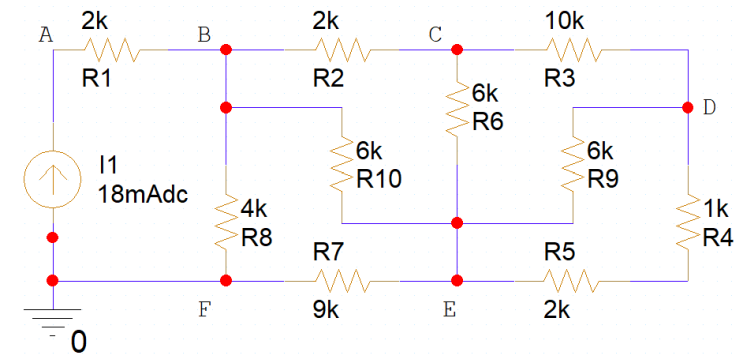
\includegraphics[width=0.7\textwidth]{graphics/ex3/f2.PNG}
    \caption{Mạch ban đầu}
\end{figure}

\subsection{Vẽ lại mạch}

\begin{figure}[!htbp]
    \centering
    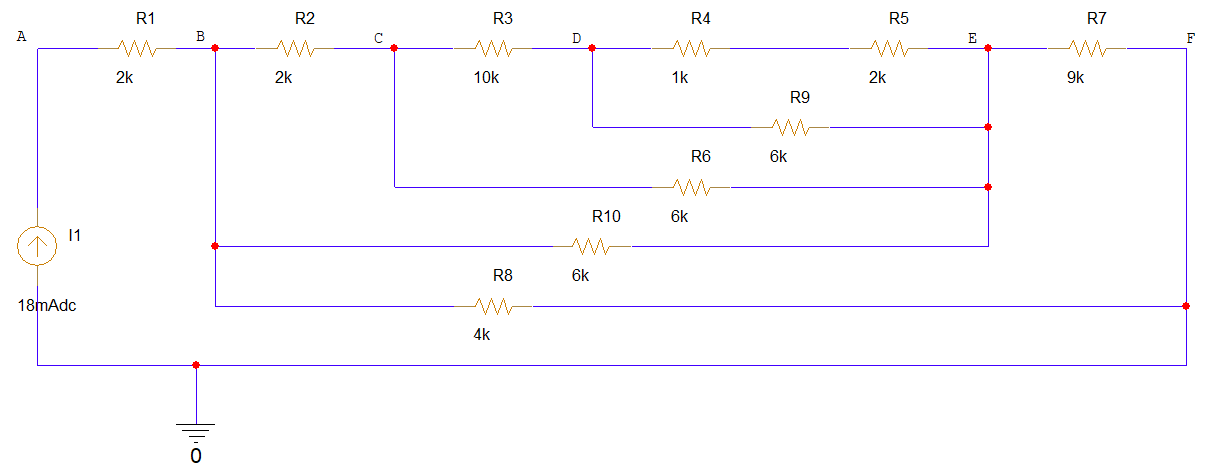
\includegraphics[width=1\textwidth]{graphics/ex3/f1.PNG}
    \caption{Mạch tương đương}
\end{figure}

\pagebreak

\subsection{Tính toán}

\begin{align*}
    R_{DE} & = \frac{(R_4 + R_5)R_9}{R_4 + R_5 + R_9} = 2 \text{k}\Omega                            \\
    R_{CE} & = \frac{(R_{DE} + R_3)R_6}{R_{DE} + R_3 + R_6} = 4 \text{k}\Omega                      \\
    R_{BE} & = \frac{(R_{CE} + R_2) R_{10}}{R_{CE} + R_{2} + R_{10}} = 3 \, \text{k}\Omega.         \\
    R_{BF} & = \frac{(R_{BE} + R_{7}) R_{8}}{R_{BE} + R_{7} + R_{8}} = 3 \, \text{k}\Omega.         \\
    R_{AF} & = R_{1} + R_{BF} = 5 \, \text{k}\Omega.                                                \\ \\
%
    V_{AF} & = R_{AF} I_1 = 90 \, \text{V}.                                                         \\
    V_{BF} & = R_{BF}I_1 = 54 \, \text{V}.                                                          \\
    V_{EF} & = \frac{R_{7}}{R_{BE} + R_{7}} V_{BF} = 40.5 \, \text{V}.                               \\
    V_{BE} & = V_{BF} - V_{EF} = 13.5 \, \text{V}.                                                        \\
    V_{CF} & = \frac{R_{CE}}{R_{2} + R_{CE}} V_{BE} + V_{EF} = 49.5 \, \text{V}.                             \\
    V_{DF} & = \frac{R_{DE}}{R_{DE} + R_{3}} \frac{R_{CE}}{R_{2} + R_{CE}} V_{BE} + V_{EF} = 42 \, \text{V}. \\
\end{align*}
%
Cho \(V_F = 0\)
%
\begin{align*}
    V_{A} & = 90 \, \text{V}.   \\
    V_{B} & = 54 \, \text{V}.   \\
    V_{C} & = 49.5 \, \text{V}. \\
    V_{D} & = 42 \, \text{V}.   \\
    V_{E} & = 40.5 \, \text{V}. \\
\end{align*}

\pagebreak

\subsection{Mô phỏng}

\begin{figure}[!htbp]
    \centering
    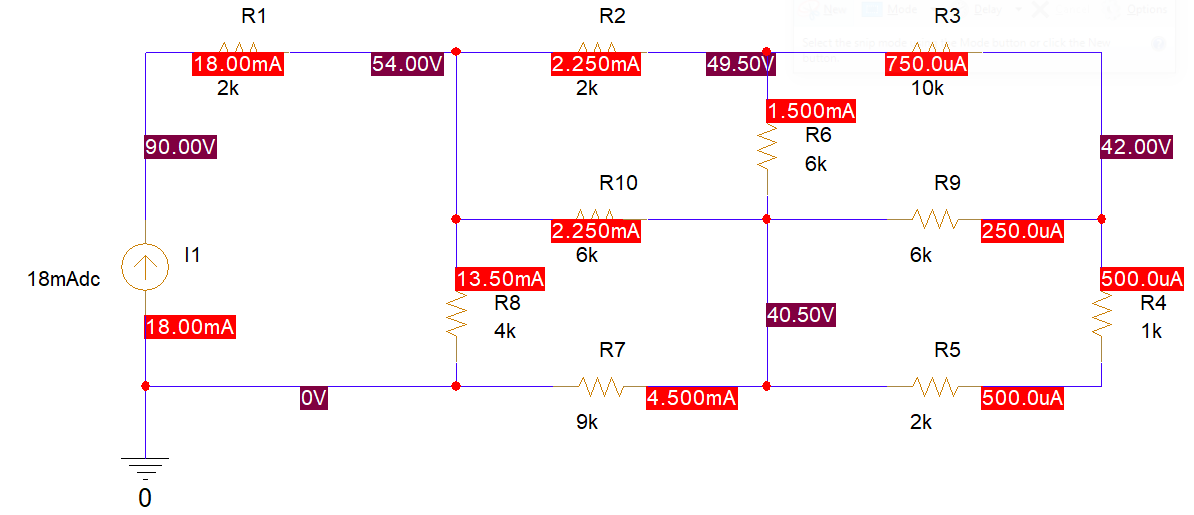
\includegraphics[width=1\textwidth]{graphics/ex3/f3.PNG}
    \caption{Mạch ban đầu}
    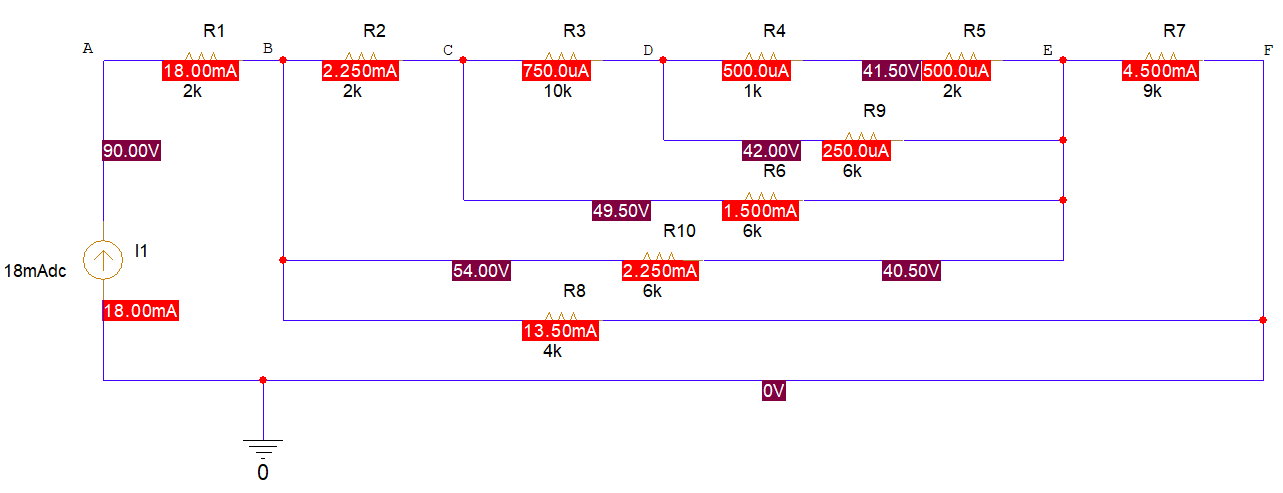
\includegraphics[width=1\textwidth]{graphics/ex3/f4.PNG}
    \caption{Mạch tương đương}
\end{figure}

